\documentclass[10pt, conference, compsocconf]{IEEEtran}
\bibliographystyle{IEEEtran}





\usepackage{cite}
\usepackage{url}
\usepackage[pdftex]{graphicx}
\graphicspath{{pics/}}
\DeclareGraphicsExtensions{.pdf,.png}

\usepackage{fixltx2e}


\usepackage{algorithm}
\usepackage{algorithmic}
% algorithmic.sty can be obtained at:
% http://www.ctan.org/tex-archive/macros/latex/contrib/algorithms/
% algorithmicx.sty package by Szasz Janos:
% http://www.ctan.org/tex-archive/macros/latex/contrib/algorithmicx/




% *** ALIGNMENT PACKAGES ***
%
%\usepackage{array}
% Frank Mittelbach's and David Carlisle's array.sty patches and improves
% the standard LaTeX2e array and tabular environments to provide better
% appearance and additional user controls. As the default LaTeX2e table
% generation code is lacking to the point of almost being broken with
% respect to the quality of the end results, all users are strongly
% advised to use an enhanced (at the very least that provided by array.sty)
% set of table tools. array.sty is already installed on most systems. The
% latest version and documentation can be obtained at:
% http://www.ctan.org/tex-archive/macros/latex/required/tools/



%\usepackage{eqparbox}
% Also of notable interest is Scott Pakin's eqparbox package for creating
% (automatically sized) equal width boxes - aka "natural width parboxes".
% Available at:
% http://www.ctan.org/tex-archive/macros/latex/contrib/eqparbox/





% *** SUBFIGURE PACKAGES ***
%\usepackage[tight,footnotesize]{subfigure}
% subfigure.sty was written by Steven Douglas Cochran. This package makes it
% easy to put subfigures in your figures. e.g., "Figure 1a and 1b". For IEEE
% work, it is a good idea to load it with the tight package option to reduce
% the amount of white space around the subfigures. subfigure.sty is already
% installed on most LaTeX systems. The latest version and documentation can
% be obtained at:
% http://www.ctan.org/tex-archive/obsolete/macros/latex/contrib/subfigure/
% subfigure.sty has been superceeded by subfig.sty.



%\usepackage[caption=false]{caption}
%\usepackage[font=footnotesize]{subfig}

\usepackage{caption}
\usepackage[font=footnotesize,caption=false]{subfig}
% subfig.sty, also written by Steven Douglas Cochran, is the modern
% replacement for subfigure.sty. However, subfig.sty requires and
% automatically loads Axel Sommerfeldt's caption.sty which will override
% IEEEtran.cls handling of captions and this will result in nonIEEE style
% figure/table captions. To prevent this problem, be sure and preload
% caption.sty with its "caption=false" package option. This is will preserve
% IEEEtran.cls handing of captions. Version 1.3 (2005/06/28) and later 
% (recommended due to many improvements over 1.2) of subfig.sty supports
% the caption=false option directly:
%\usepackage[caption=false,font=footnotesize]{subfig}
%
% The latest version and documentation can be obtained at:
% http://www.ctan.org/tex-archive/macros/latex/contrib/subfig/
% The latest version and documentation of caption.sty can be obtained at:
% http://www.ctan.org/tex-archive/macros/latex/contrib/caption/



% correct bad hyphenation here
%\hyphenation{op-tical net-works semi-conduc-tor}


\begin{document}

\title{A NUMA-aware fine grain parallelization framework for multi-core architecture}


% author names and affiliations
% use a multiple column layout for up to two different
% affiliations

\author{\IEEEauthorblockN{Corentin Rossignon}
\IEEEauthorblockA{Total - E\&P\\
CSTJF\\
Pau, France\\
corentin.rossignon@total.com}
\and
\IEEEauthorblockN{Pascal H\'enon}
\IEEEauthorblockA{Total - E\&P\\
CSTJF\\
Pau, France\\
pascal.henon@total.com}
\and
\IEEEauthorblockN{Olivier Aumage}
\IEEEauthorblockA{Inria\\
Runtime project team\\
Bordeaux, France\\
olivier.aumage@inria.fr}
\and
\IEEEauthorblockN{Samuel Thibault}
\IEEEauthorblockA{Universit\'{e} Bordeaux I\\
Runtime project team\\
Bordeaux, France\\
samuel.thibault@labri.fr}
}


% make the title area
\maketitle


\begin{abstract}
 We present some solutions to handle two problems commonly encountered when dealing with fine grain parallelization
 on multi-core architecture: Expressing algorithms using a task grain size suitable for the hardware and 
 minimizing the time penalty due to Non Uniform Memory Accesses.
 To evaluate the benefit of our work we present some experiments on the fine grain parallelization of an iterative solver 
  for sparse linear systems with some comparisons with the Intel TBB approach.
\end{abstract}

\begin{IEEEkeywords}
task flow; scheduler; aggregation; fine-grain parallelism; NUMA
\end{IEEEkeywords}


\IEEEpeerreviewmaketitle


%=========================================================
\section{Introduction}
%=========================================================
\input{chapter_introduction}

%=========================================================
\section{Problem Statement}\label{sec:problem}
%=========================================================
%\begin{itemize}
%  \item Explain task flow based parallelization
%  \item Cite some task based software(StarPU \cite{starpu}, TBB \cite{Intel::TBB}, OpenMP 3.0 \cite{openmp08}, Cilk).
%  \item task size problem
%  \item no major improvement since Cilk
%\end{itemize}

The principle of using tasks to express the potential application
parallelism in an abstract way, independent from available hardware
resources, was once popularized by tools such as
Cilk~\cite{cilk}. The widespread availability of multi-core processors
recently revived the popularity of task scheduling frameworks~\cite{taskscomparison} as
exemplified by tools such as Intel TBB~\cite{Intel::TBB} and
OpenMP~3.0's task support~\cite{openmptasks} for regular multi-core platforms,
or StarSs/OmpSs derivatives~\cite{ompss} as well as StarPU~\cite{starpu} and
X-Kaapi~\cite{xkaapi} for heterogeneous platforms. 

Most frameworks for multi-core platforms don't handle memory locality, some
try to improve data locality between tasks by leaving the user with the choice of the next task
to schedule (e.g., {\em continuation} in TBB). In the case of a task scheduler for
heterogeneous platforms, data need to be moved to the target platform. Therefore, in this case, the
scheduler must know which data are used by each task to move them at the right
time. Unfortunately none of these schedulers care about NUMA in their scheduling algorithms to reduce the overhead 
of data movement.

Several related works have been conducted in the past to address the
issue of adapting the task grain size to the amount of available
computing units. Many related works partially address this
grain size issue by promoting cache-oblivious techniques for a specific class of
applications such as recursive, divide-and-conquer
codes or recursively partitioned loops~\cite{unifieddataflow,Intel::TBB,cilk,xkaapi,taskscomparison}.

Works such as the SCOOPP framework~\cite{scoopp} provides means for the applications to control
the task grain size. However, the grain size selection issue is still up to
the application programmer. 

On the theoretical side, general task scheduling has been heavily studied for
a long time now~\cite{Khan94acomparison,heft}. Works on task grain
adaptiveness have been scarcer, but do exist. The work presented in this
paper is built on grain-packing~\cite{GeY96} and task clustering~\cite{triplet}
past works.


%=========================================================
\section{Task-grain tuning through Guided Aggregation}\label{sec:proposal}
%=========================================================
%  \begin{itemize}
%    \item Talk about existent framework (X-Kaapi, Capsule). (OK)
%    \item Talk about our solution Taggre and his back-end.
%    \item Define Aggregation constrains
%    \item Describe Aggregate algorithm
%    \item little section on aggregate overhead
%  \end{itemize}

To solve the granularity problem, several possible approaches exist. We
could enable task parallelism only when cores are idle. For example,
% ST: TODO: X-Kaapi est un logiciel, pas une équipe. Il faut donc
% accorder à la 3e personne.
X-Kaapi~\cite{xkaapi} uses this approach with its {\em adaptive task model}.
This is a very good solution with parallel loops or tree task flow.
However, in the general case, the user needs to define a function that
splits the task flow graph into two complete parallel parts, which is
not always possible.

Another possible approach, as given by Capsules~\cite{capsules},
requires the user to define several grain sizes. The 
runtime then chooses which grain best matches the current situation. The
application programmer must therefore design his/her application while
having these multiple granularity levels in mind, which may prove
difficult to realize or express in an abstract way in the code.

Our approach is different. From the finest-grained DAG, we build a
coarse-grained DAG after the machine topology layout and the run-time
state using an {\em aggregate operator} on subsets of tasks. 
Our default aggregate operator just serializes the function called within all 
merged tasks. But the aggregate operator itself is user programmable by overloading the aggregate method 
of our task class. Indeed, it is often interesting to redefine this
operator: For example, instead of calling sequentially several functions that depend on a parameter 
$i$, it is more efficient to use a single function call that loops on the list of $i$ parameters.

Several possible aggregate operators are experimented later in this paper.
% We have chosen to let the programmer do the aggregation of two tasks because he
% can then optimize the tasks execution to preserve data locality.
Those aggregate operators are called from a dedicated framework
called Taggre, which interfaces with existing low-level task
schedulers. Taggre expects a fine grain task DAG as input. It then
returns a coarser DAG as the result of applying the selection of aggregate
operators on the contents of the fine-grain DAG.

%-------------------------------
\subsection{Aggregate operator algorithms}
As a proof of concept, we have defined several heuristics that
coarse the DAG to change the task grain size.
%% coarsening the grain size of task DAGs.
Multiple heuristics may be
chained together to further coarsen the DAG. In Taggre, each algorithm is
thus designated by a letter. The sequence of selected letters is
called the  {\bf Coarse String}. For example, the Coarse String
% ST: TODO: expliquer aussi la notation 4F(32) qui est utilisée plus loin
% dans les tableaux.
``SD(300)F(32)'' means the call of Sequential algorithm, followed
by the Depth Front algorithm with parameter 300 and finally by the
Front algorithm with parameter 32. The parameters are
algorithm-dependent.

\subsubsection{Sequential (S)}
This is the most straightforward algorithm. We aggregate
tasks having a single predecessor with their predecessor, if such
a predecessor has a single successor (Fig.~\ref{fig:S_algo}).
%   (-_-)   %
\begin{figure}[t!]
  \centering
  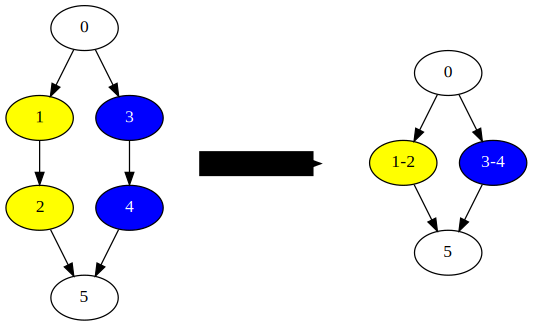
\includegraphics[width=3in]{algo_S}
  \caption{Example of aggregation with S algorithm}
  \label{fig:S_algo}
\end{figure}


\subsubsection{Front (F)}
This algorithm takes one argument which is the maximum number of
tasks per depth level. We call this number $N$. The basic idea of
this algorithm is to limit the number of simultaneously available
tasks and thus to limit the oversubscription of computing units.
To do this, the Front algorithm implements a breadth-first traversal
of the DAG. During the traversal, it aggregates tasks of same
depth to build up to the maximum of $N$ coarse tasks of similar computation
time (e.g., grain size) per depth (Fig.~\ref{fig:F_algo}).

\begin{figure}[t!]
  \centering
  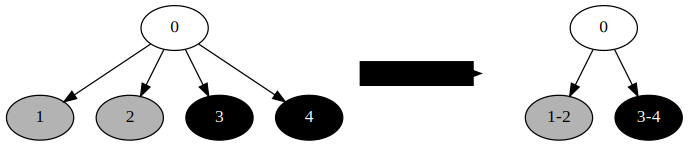
\includegraphics[width=3in]{algo_F2}
  \caption{Example of aggregation with the F algorithm and parameter 2}
  \label{fig:F_algo}
\end{figure}


\subsubsection{Depth Front (D)}
This algorithm expects one argument which is the maximum number of
fine grain tasks aggregated into a coarse grain task. We call this
number $M$.
The main idea of this algorithm is to aggregate a task with some
of its descendants, up to the limit $M$. For that, the algorithm
performs a breadth-first traversal of the descendants of a task to
aggregate up to $M$ tasks together. However, during the traversal, each new
level encountered is sorted, from the task having the highest
number of predecessors in the current aggregate being built, to
the task having the least predecessors in this aggregate. The
rationale of this heuristics is to favor aggregating tasks that
are more tightly connected in the DAG (Fig.~\ref{fig:D_algo}).


The first loop of Algorithm~\ref{depth_front_algo} is a loop for each
level of the coarsened DAG.

The second loop is a loop over tasks of the same level in coarsened DAG.
Other tasks will be aggregated to these tasks in the third loop, we call them
{\em Master} and they will be kept in the final DAG.

The third loop is the aggregation loop, we aggregate tasks descendants of
the {\em Master} task to it.

\begin{algorithm}
  \caption{Depth Front}
  \label{depth_front_algo}
  \begin{algorithmic} 
    \REQUIRE $M$, DAG
    \STATE Ready = empty list
    \STATE put root tasks of DAG in Ready
    \WHILE{Ready not empty}
    \STATE Depth = Ready
    \STATE Ready = empty list
    \WHILE{Depth is not empty}
    \STATE Master = pop first from Depth
%    \STATE DAG\_tmp = DAG.clone()
    \STATE Release = empty list
    \STATE put Master in Release
    \STATE count: 0
    \WHILE{$count < M$ AND Release is not empty}
    \STATE Next = pop first from Release
    \STATE count++
    \STATE aggregate Master and Next
    \STATE put tasks released by Next in Release, sorted by
    \STATE \quad number of precedence of Master
    \ENDWHILE
    \STATE put tasks released by Master in Depth
    \ENDWHILE
    \STATE put tasks released by Depth in Ready
    \ENDWHILE
  \end{algorithmic}
\end{algorithm}

\begin{figure}[t!]
  \centering
  \includegraphics[width=3in]{algo_2}
  \caption{Example of aggregation with D algorithm and parameter 4}
  \label{fig:D_algo}
\end{figure}

\subsubsection{Continuation Oriented (C)}
The Continuation Oriented algorithm is an aggregation method which improves 
serial accesses to data inside an aggregated task. For a 3D cube,
it's equivalent to putting tasks with the same (x,y) coordinates together.

%% To begin, the user must register an identifier on each tasks with the constraint
%% of following identifier have data that follow. Then the Cache Oriented algorithm
%% aggregate tasks with continuous identifier if a dependency exist between them.
%% This algorithm couldn't be use on all DAG, in some of them, this aggregation
%% will form cycle dependencies and the coarsed graph can't be execute.


%=========================================================
\section{Application to a sparse linear solver}\label{sec:appli}
%=========================================================
% ST: TODO: expliquer ce que sont les valeurs en gras

%\begin{itemize}
%  \item Explain k in ILU(k) and impact on task size
%  \item Factorization have little data reuse
%  \item Solve don't have data reuse
%  \item Facto time, aggregation improve speed-up but less than domain decomposition
%  \item Solve time, same as facto
%  \item Agg time, need to be considerate, could be avoid by many facto/solve or compute offline if possible
%  \item We have a data locality problem and task aren't big enough
%  \item benefit of task scheduling in load balancing
%\end{itemize}

To illustrate the benefit of aggregation, we propose to study the parallelization of an iterative 
solver for sparse linear system. 
%A popular iterative method a GMRES preconditioned 
%sparse linear algebra, the GMRES with an ILU(k) preconditionner~\cite{Saad96IMSLS}.
%In this GMRES we have two major steps, the first step is the {\em ILU matrix factorization}
%and the second step is the {\em triangular solve}.
A popular approach to solve large sparse linear systems of equation is a Krylov
method (like GMRES or Conjugate Gradient) preconditioned by an incomplete
factorization (see~\cite{Saad96IMSLS}).
This is often the most time consuming part of a numerical simulation.
In this method there is two major operations, the first step is the {\em ILU matrix factorization}
and the second step is the {\em triangular solve}.
%The usual way to parallelize those kind of solver is to use a weaker form of
%the preconditioner in parallel by preconditioning subdiagonal block of the
%matrix: the subdiagonal block are usually obtained thank to a partition of
%the adjacency graph of the matrix.
Outside the preconditioner, the operations required in a Krylov method are
mostly BLAS1 operations and matrix vector products which naturally dealt with
parallel loop splitting.
In our experiments, we focus on the fine grain parallelization of
the ILU preconditioner; that is to say the factorization of the matrix (done once per system solve) and
the triangular system solves (done once at each iteration of the system solve).


Both of those algorithms (factorization and triangular solve) can naturally be represented as a task graph. For example in the factorization 
a task corresponds to the factorization of a matrix row and the dependencies are directly given by the non-zero pattern of the matrix.
%Indeed, the factorization of row $i$ can be done only when all the rows which index corresponds to an entry in the non-zero array of row $i$ before the diagonal have been factorized.
Indeed, to factorize the row $i$, we need to factorize all the rows $j$ lower than $i$ 
% which have an entry in the non-zero array of row $i$.
such that the entry $(i,j)$ is non-zero.
Therefore the DAG description is easily built from the non-zero pattern of the matrix:
the task $i$ corresponds to row $i$ of the matrix, the predecessor tasks of task $i$ are given by the column index of non-zero coefficients before the diagonal in row $i$
 and successor tasks of task $i$ are given by the row index of non-zero coefficients below the diagonal in the column $i$.

Incomplete factorization and associated triangular solve of a sparse matrix
is a problem that is well representative of the difficulty that one can encounter
with fine-grain parallelization: The fine grain description of these algorithms
is natural, but in practice, a straightforward task based parallelization using TBB or
OpenMP does not deliver good speed-ups because of the very low computational cost of
a task and the NUMA effect when accessing the coefficient of the matrix and vector.
In the experiment results, we will evaluate our programming model on those algorithms.

Our testing machine is composed of two Intel Xeon X5570 (Nehalem)
4-core sockets with 24\,GB RAM (12\,GB per socket) running Red Hat Enterprise Linux 5.2
with a Linux kernel 2.6.18.
The compiler used is Intel C++ compiler XE 13 with level 3
optimizations. The back-end task scheduling runtime is Intel TBB. We obtain comparable
results using OpenMP tasks.

We perform the tests on two linear systems. The first one, Cube\_100, is a
system obtained from a 7 points discretization scheme (e.g., finite volume) of regular 
3D cubes with 100 points along each dimension. 
It is a scalar system; each row of the matrix is a vector of coefficients stored in double precision. 
The second one, SPE10, corresponds to a 7 points discretization of a reference problem from petroleum industry~\cite{spe10}. 
In this case each entry of the matrix is a small dense block $(3,3)$ of coefficients stored in double precision.
Due to the geometry of the problem, for Cube\_100, the task dependency graph is very regular whereas it is an irregular one in the SPE10 case.
The characteristics of the matrices are listed in Table~\ref{matrices}.

\begin{table}[!h]
  \renewcommand{\arraystretch}{1.3}
  \caption{Matrices used in tests.}
  \label{matrices}
  \centering
  \begin{tabular}{|c||c|c|}
    \hline
    Name & Cube\_100 & SPE10\\
    \hline
    \hline
%    Type & Synthetic & Real Life Case\\
%    \hline
    Rows ($n$) & 1,000,000 & 3,283,263\\
    \hline
    Number of non-zeros ($nnz$) & 6,940,000 & 67,303,269\\
    \hline
    Entries of the matrix & Scalars & $(3,3)$ dense blocks\\
    \hline
  \end{tabular}
\end{table}

Each fine grain task performs one elementary line operation. SPE10
tasks weight 2-5 times more than Cube\_100 tasks. However, both
cases generate approximately 1 million tasks each.

The test protocol is the following:
\begin{itemize}
\item Each test is run three times, the final retained result is
  computed as the average of the three measured results. For each
  test, we collect three different timings:
  factorization time, triangular solve time, and aggregation time.

\item We perform the tests on a single socket (using
      {\em numactl --cpunodebind}) and on two sockets.

  % OA: je pense qu'un mot d'explication sur l'ordering sera
  % necessaire
  
\item We test two orderings (set of row/column permutations): A {\em natural} ordering which corresponds to no
      modification on matrix structure where unknowns are sequentially
      ordered by plane along the geometric z axis
      (this leads to a perfect seven diagonals pattern for Cube\_100)
      and a {\em nested dissection}~\cite{Saad96IMSLS} ordering which exposes more parallelism.

  % ST: TODO: expliquer brièvement ce que sont les natural et nest
  % dissection orderings.
  % ST: TODO: expliquer pourquoi ça n'a pas de sens d'appliquer
  % D() au cas nested dissection.

\item We test three levels of ILU(k) fill: 0, 1 and 2.
      The level $k$ of ILU(k) preconditioner determines the level of fill of
      the matrix. In others words, computation per line and the number of dependencies
      between tasks grow up with a greater $k$. Table~\ref{tab:edges} gives the number of edges resulting in the DAG of the factorization 
      (triangular solve DAG has a similar number of edges) for ILU$(0)$, ILU$(1)$ and ILU$(2)$. Subsection \ref{precond_step} will also give some features on the cost of a computational task (one row factorization) 
      depending on the ILU level of fill parameter.  

\item For the parameterized aggregation heuristics, we select the
      parameter values leading to the best performance result. With
      natural ordering, we can use the Cache Oriented algorithm because of
      particular DAG structure. With nested dissection ordering, the Cache Oriented algorithm
      can't be used, so we use the Depth Front algorithm with a high value.
\end{itemize}

In all tables, best results are represented in bold.


\begin{table}[!h]
  \renewcommand{\arraystretch}{1.3}
  \caption{Number of edges in computation DAG}
  \label{tab:edges}
  \centering
  \begin{tabular}{|c|c||c|}
    \hline
     Matrix & ILU & Edges\\
     \hline
     \hline
     CUBE\_100 & ILU(0) & 2,970,000\\
     Natural   & ILU(1) & 5,910,300\\
     ordering  & ILU(2) & 10,761,498\\
     \hline
     SPE10     & ILU(0) & 2,970,000\\
     Natural   & ILU(1) & 5,910,300\\
     ordering  & ILU(2) & 11,357,865\\
     \hline
   \end{tabular}
\end{table}
%-------------------------------

% OA: TODO: relire la section ``domain decomposition'' pour l'instant
% elle est trop courte.


%-------------------------------
% \subsection{Domain decomposition}
% With domain decomposition we have a total parallel application,
% in this way we can estimate an upper limit we can reach without
% domain decomposition.

% CR: J'enlève la decomposition de domaine car l'article est maintenant
% centré sur les problèmes NUMA

% ST: TODO: Pourquoi avoir enlevé les mesures ? sans cela on se
% demande à quoi sert la section (surtout quand on ne connait pas
% GMRES). Ou alors expliquer clairement pourquoi on ne les met pas.

%% \begin{table}[!h]
%%   \renewcommand{\arraystretch}{1.3}
%%   \caption{Result of domain decomposition with MPI in ILU(0)}
%%   \label{tab:domain}
%%   \centering
%%   \begin{tabular}{|c|c||c|c|c|c|}
%%     \hline
%%     Matrix & Method & Sequential & 4 domains & 8 domains\\
%%     &     &  (second)  & \multicolumn{2}{c|}{(speed-up)}\\
%%     \hline
%%     \hline
%%     \hline
%%     CUBE\_100   & Facto & 0.056 & 3.83 & 7.45\\
%%     No ordering & Solve & 0.923 & 2.14 & 4.23\\
%%     \hline
%%     CUBE\_100         & Facto & 0.120 & 3.71 & 7.14\\
%%     Nested dissection & Solve & 1.305 & 2.12 & 3.88\\
%%     \hline
%%     \hline
%%     SPE10       & Facto & 0.189 & 2.47 & 4.83\\
%%     no ordering & Solve & 9.884 & 1.99 & 3.82\\
%%     \hline
%%     SPE10             & Facto & 0.263 & 3.40 & 6.58\\
%%     Nested dissection & Solve & 10.24 & 1.99 & 3.82\\
%%     \hline
%%   \end{tabular}
%% \end{table}


%-------------------------------
\subsection{ILU(k) Factorization Step}
\label{precond_step}
The first test series is performed on the ILU(k) factorization step
on a single 4-core socket (Tables~\ref{tab:tbb:4:facto:no},~\ref{tab:tbb:4:facto:nested}).

% ST: TODO: mentionner que ça consiste ici en trois phases de
% préconditionnement: ILU(0), ILU(1), ILU(2), et indiquer brièvement la
% différence entre ces phases. Tout le monde ne connait pas
% GMRES, loin de là:)
With aggregation disabled the task-parallel ILU(0) factorization is always
slower than the sequential version. This is due to the additional cost
of task management. Tasks duration for CUBE\_100 in ILU(0) is only $50\,ns$ and 
$240\,ns$ for SPE10, but one task
management duration is approximately $500\,ns$. In ILU(2), tasks are bigger, their
duration is $600\,ns$ for CUBE\_100 and $1.7\,\mu{s}$ for SPE10 but it's
not bigger enough to consider task management negligible.
Another important aspect of the ILU factorization and triangular solve is that on our testbed machine 
the algorithm speed-up is bounded by the memory bandwidth: Therefore the maximum theoretical speed-up achievable 
by such algorithms on several cores is less than the number of cores used. 

With aggregation enabled and {\em CD(4)} coarse strategy string, we now reduce the number
of tasks to 2,500 with a task duration 400 times bigger.
In ILU(0) we achieve a moderate speed-up of 2. ILU(2) factorization achieves a
better speed-up of 3. The Front algorithm is not as effective as
the Depth Front in this test case, because it doesn't aggregate tasks
with continuous lines, which cause many cache misses.

% ST: TODO: Que veut dire contiguous data?
% ST: TODO: est-ce que ça aide de faire plusieurs D(4) ? En faire
% plus aurait-il aidé plus ? Discuter de quand s'arrêter ?

With the Front algorithm ({\em F(32)}) in ILU(0) with natural ordering,
%tasks at the begin and the end of the DAGs are not aggregated,
we aggregate a maximum of 157 tasks together and, on average, we aggregate only 53 tasks.

\begin{table}[!h]
  \renewcommand{\arraystretch}{1.3}
  \caption{Results on the ILU(k) factorization step on a single 4-core
    socket with TBB with natural ordering.}
  \label{tab:tbb:4:facto:no}
  \centering
  \begin{tabular}{|c|c||c|c|c|c|}
    \hline
    Matrix & ILU & Sequential & No agg. & F(32) & CD(4)\\
    &     &  (second)  & \multicolumn{3}{c|}{(speed-up)}\\
    \hline
    \hline
    \hline
    & ILU(0) & 0.056 & 0.20 & 1.06 & 2.23\\
    CUBE\_100 & ILU(1) & 0.142 & 0.46 & 1.54 & 2.81\\
    & ILU(2) & 0.611 & 1.30 & 2.58 & {\bf 3.47}\\
    \hline
    & ILU(0) & 0.262 & 0.65 & 1.89 & 3.09\\
    SPE10     & ILU(1) & 0.721 & 1.39 & 2.30 & 3.22\\
    & ILU(2) & 1.936 & 1.87 & 2.19 & 3.32\\
    \hline
  \end{tabular}
\end{table}


\begin{table}[!h]
  \renewcommand{\arraystretch}{1.3}
  \caption{Results on the ILU(k) factorization step on a single 4-core
    socket with TBB with nested dissection ordering.}
  \label{tab:tbb:4:facto:nested}
  \centering
  \begin{tabular}{|c|c||c|c|c|c|}
    \hline
    Matrix & ILU & Sequential & No agg. & F(32) & D(400)\\
    &     &  (second)  & \multicolumn{3}{c|}{(speed-up)}\\
    \hline
    \hline
    & ILU(0) & 0.129 & 0.46 & 2.17 & 2.26\\
    CUBE\_100 & ILU(1) & 0.495 & 1.29 & 1.70 & 2.78\\
    & ILU(2) & 0.828 & 1.74 & 1.94 & {\bf 3.12}\\
    \hline
    & ILU(0) & 0.276 & 0.74 & 1.93 & 2.16\\
    SPE10     & ILU(1) & 1.375 & 1.98 & 1.67 & 2.82\\
    & ILU(2) & 2.247 & 2.43 & 1.85 & {\bf 3.12}\\
    \hline
  \end{tabular}
\end{table}

With two 4-core sockets (Tables~\ref{tab:tbb:8:facto:no},~\ref{tab:tbb:8:facto:nested}), the parallel
ILU(0) again performs slower than sequential execution when
aggregation is disabled. With aggregation enabled, the ILU(0)
achieves a speed-up of 3. ILU(2) achieves a speed-up of 6.2.

\begin{table}[!h]
  \renewcommand{\arraystretch}{1.3}
  \caption{Results on the ILU(k) factorization step on two 4-core
    sockets with TBB with natural ordering.}
  \label{tab:tbb:8:facto:no}
  \centering
  \begin{tabular}{|c|c||c|c|c|c|}
    \hline
    Matrix & ILU & Sequential & No agg. & F(32) & CD(4)\\
    &     &  (second)  & \multicolumn{3}{c|}{(speed-up)}\\
    \hline
    \hline
    \hline
    & ILU(0) & 0.056 & 0.28 & 1.27 & 2.54\\
    CUBE\_100 & ILU(1) & 0.143 & 0.65 & 1.89 & 3.79\\
    & ILU(2) & 0.612 & 1.47 & 3.06 & 3.91\\
    \hline
    & ILU(0) & 0.260 & 0.97 & 2.48 & 3.78\\
    SPE10     & ILU(1) & 0.771 & 2.24 & 3.80 & 5.72\\
    & ILU(2) & 2.006 & 3.37 & 3.97 & {\bf 6.21}\\
    \hline
  \end{tabular}
\end{table}


\begin{table}[!h]
  \renewcommand{\arraystretch}{1.3}
  \caption{Results on the ILU(k) factorization step on two 4-core
    sockets with TBB with nested dissection ordering.}
  \label{tab:tbb:8:facto:nested}
  \centering
  \begin{tabular}{|c|c||c|c|c|c|}
    \hline
    Matrix & ILU & Sequential & No agg. & F(32) & D(400)\\
    &     &  (second)  & \multicolumn{3}{c|}{(speed-up)}\\
    \hline
    \hline
    & ILU(0) & 0.127 & 0.41 & 3.10 & 3.31\\
    CUBE\_100 & ILU(1) & 0.483 & 1.31 & 2.70 & 4.77\\
    & ILU(2) & 0.817 & 1.96 & 3.18 & 5.46\\
    \hline
    & ILU(0) & 0.277 & 0.71 & 2.59 & 3.09\\
    SPE10     & ILU(1) & 1.452 & 2.48 & 2.81 & 5.00\\
    & ILU(2) & 2.347 & 3.29 & 3.12 & {\bf 5.57}\\
    \hline
  \end{tabular}
\end{table}

%-------------------------------
\subsection{Triangular Solve Step}\label{subsec:solve}

The triangular solve step is itself composed of two parts: A
{\em forward} substitution followed by a {\em backward}
substitution. The DAG of the forward substitution is identical to
the DAG of the factorization step mentioned in the previous section.
Thus we can reuse the same coarse
DAG. In our test cases, the DAG of the backward substitution part is
the transpose of the DAG of the forward substitution. Here again,
the factorization coarse DAG can thus straightforwardly be reused.
In total we have twice more tasks in triangular solve than in factorization.

The weight of operations done in triangular solve elementary tasks
is lighter than their factorization task counterparts.
%% and these tasks need to access to more data..
Tests on a
single 4-core socket (Tables~\ref{tab:tbb:4:solve:no},~\ref{tab:tbb:4:solve:nested})
show that the parallel triangular solve is always slower than
the sequential version with task aggregation disabled. With
aggregation enabled, we obtain a speedup of~2.

% ST: TODO: idéalement il faudrait que ces deux tables se retrouvent
% côte à côte dans la version finale.
\begin{table}[!h]
  \renewcommand{\arraystretch}{1.3}
  \caption{Results on the Triangular Solve step on a single 4-core
    socket with TBB with natural ordering.}
  \label{tab:tbb:4:solve:no}
  \centering
  \begin{tabular}{|c|c||c|c|c|c|}
    \hline
    Matrix & ILU & Sequential & No agg. & F(32) & CD(4)\\
    &     &  (second)  & \multicolumn{3}{c|}{(speed-up)}\\
    \hline
    \hline
    & ILU(0) & 0.092 & 0.23 & 0.88 & 1.90\\
    CUBE\_100 & ILU(1) & 0.117 & 0.27 & 0.82 & 1.97\\
    & ILU(2) & 0.163 & 0.34 & 0.92 & 2.05\\
    \hline
    & ILU(0) & 0.219 & 0.40 & 1.08 & 1.93\\
    SPE10     & ILU(1) & 0.353 & 0.62 & 1.37 & 2.22\\
    & ILU(2) & 0.554 & 0.85 & 1.58 & {\bf 2.39}\\
    \hline
  \end{tabular}
\end{table}

\begin{table}[!h]
  \renewcommand{\arraystretch}{1.3}
  \caption{Results of the Triangular Solve step on a single 4-core
    socket with TBB with nested dissection ordering.}
  \label{tab:tbb:4:solve:nested}
  \centering
  \begin{tabular}{|c|c||c|c|c|c|}
    \hline
    Matrix & ILU & Sequential & No agg. & F(32) & D(400)\\
    &     &  (second)  & \multicolumn{3}{c|}{(speed-up)}\\
    \hline
    \hline
    & ILU(0) & 0.107 & 0.20 & 1.19 & 1.34\\
    CUBE\_100 & ILU(1) & 0.150 & 0.31 & 0.94 & 1.39\\
    & ILU(2) & 0.171 & 0.34 & 0.95 & 1.50\\
    \hline
    & ILU(0) & 0.249 & 0.37 & 1.39 & 1.52\\
    SPE10     & ILU(1) & 0.430 & 0.65 & 1.32 & 1.77\\
    & ILU(2) & 0.500 & 0.72 & 1.35 & {\bf 1.89}\\
    \hline
  \end{tabular}
\end{table}

On two 4-core sockets
(Tables~\ref{tab:tbb:8:solve:no},~\ref{tab:tbb:8:solve:nested}), with
task aggregation disabled, only the SPE10 test achieves a speedup
greater than 1. With aggregation enabled, a speedup of 2.52 is
achieved on ILU(0) and a speedup of 4.14 is achieved on ILU(2).

\begin{table}[!h]
  \renewcommand{\arraystretch}{1.3}
  \caption{Results of the Triangular Solve step on two 4-core sockets with
    TBB with natural ordering.}
  \label{tab:tbb:8:solve:no}
  \centering
  \begin{tabular}{|c|c||c|c|c|c|}
    \hline
    Matrix & ILU & Sequential & No agg. & F(32) & CD(4)\\
    &     &  (second)  & \multicolumn{3}{c|}{(speed-up)}\\
    \hline
    \hline
    & ILU(0) & 0.092 & 0.27 & 1.27 & 2.44\\
    CUBE\_100 & ILU(1) & 0.123 & 0.35 & 1.54 & 2.82\\
    & ILU(2) & 0.174 & 0.45 & 1.40 & 2.98\\
    \hline
    & ILU(0) & 0.219 & 0.53 & 1.63 & {\bf 2.52}\\
    SPE10     & ILU(1) & 0.408 & 0.96 & 2.39 & 3.77\\
    & ILU(2) & 0.658 & 1.38 & 2.79 & {\bf 4.14}\\
    \hline
  \end{tabular}
\end{table}


\begin{table}[!h]
  \renewcommand{\arraystretch}{1.3}
  \caption{Results of the Triangular Solve step on two 4-core
    sockets with TBB with nested dissection ordering.}
  \label{tab:tbb:8:solve:nested}
  \centering
  \begin{tabular}{|c|c||c|c|c|c|}
    \hline
    Matrix & ILU & Sequential & No agg. & F(32) & D(400)\\
    &     &  (second)  & \multicolumn{3}{c|}{(speed-up)}\\
    \hline
    \hline
    & ILU(0) & 0.107 & 0.18 & 1.41 & 1.67\\
    CUBE\_100 & ILU(1) & 0.156 & 0.32 & 1.36 & 1.92\\
    & ILU(2) & 0.180 & 0.36 & 1.37 & 2.08\\
    \hline
    & ILU(0) & 0.249 & 0.35 & 1.64 & 1.82\\
    SPE10     & ILU(1) & 0.496 & 0.80 & 2.12 & 2.71\\
    & ILU(2) & 0.578 & 0.90 & 2.19 & {\bf 2.90}\\
    \hline
  \end{tabular}
\end{table}

% In most cases, domain decomposition achieves better raw performance
% results. However, by avoiding potentially harmful domain boundaries artifacts, the
% aggregation method ensures a better overall numerical stability than the
% domain decomposition.

%-------------------------------
\subsection{Aggregation Overhead}
This section evaluates the overhead caused by the task aggregation
step for several aggregation algorithm instances. As mentioned in
the test description above, the fine-grain DAG generated from the
test cases amount to about 1 million nodes for each matrix. The 
number of edges increases when the parameter $k$ of ILU(k) preconditioner increases (see Table~\ref{tab:edges}).
This aggregation step is performed only once for each matrix. Then, the
coarsened DAG is reused as long as the sparse pattern of the matrix is unchanged.
In classical numerical simulation, the mesh on which the equations are discretized
does not change through the simulation, only the coefficients of the linear system
are changing: This means that the aggregation step is typically done only once
while the factorization and triangular solves are called a large number of times (several thousand of times).
The time spent in the task aggregation (Table~\ref{agg_time}) is then usually negligible
compared to the time spent in the factorizations and triangular solves.


On average, applying {\em CD(4)} Coarse String takes 1.5\,s on a DAG with 1 million
of nodes and applying {\em D(400)} takes 3.5\,s.

For {\em CD(4)} aggregation we won on average 0.22\,s per factorization
and 0.31\,s per triangular solve compared to not doing aggregation. So
after only 3 combinations of factorization and triangular solve, the aggregation
become profitable.

For {\em D(400)} aggregation we won in average 0.28\,s per factorization
and 0.49\,s per triangular solve. So after only 5 combinations of factorization
and triangular solve, the aggregation becomes profitable.
% ST: TODO: et donc comparer ce coût par rapport à n fois le gain
% obtenus à chaque phase.

\begin{table}[!h]
  \renewcommand{\arraystretch}{1.3}
  \caption{Aggregation overhead.}
  \label{agg_time}
  \centering
  \begin{tabular}{|c|c||c|c|c|c|}
    \hline
    Matrix & ILU & F(32) & D(400) & CD(4)\\
    &     &  \multicolumn{3}{c|}{(second)}\\
    \hline
    \hline
    \hline
    CUBE\_100  & ILU(0) & 1.534 & 2.945 & 0.908\\
    No         & ILU(1) & 1.467 & 3.032 & 1.119\\
    ordering   & ILU(2) & 1.871 & 3.705 & 1.315\\
    \hline
    CUBE\_100  & ILU(0) & 1.208 & 2.330 & N/A\\
    Nested     & ILU(1) & 2.194 & 3.224 & N/A\\
    dissection & ILU(2) & 3.182 & 3.554 & N/A\\
    \hline
    \hline
    SPE10      & ILU(0) & 1.519 & 3.239 & 1.217\\
    no         & ILU(1) & 1.542 & 3.344 & 1.527\\
    ordering   & ILU(2) & 2.019 & 4.042 & 1.918\\
    \hline
    SPE10      & ILU(0) & 1.292 & 2.541 & N/A\\
    Nested     & ILU(1) & 2.337 & 3.518 & N/A\\
    dissection & ILU(2) & 3.119 & 3.816 & N/A\\
    \hline
  \end{tabular}
\end{table}


%=========================================================
\section{NUMA}\label{sec:numa}
%=========================================================
%\begin{itemize}
%  \item Explain NUMA, and that in TBB with use only 1 NUMA node
%  \item Try of NUMA interleaved with TBB
%  \item Explain memory distribution of schema
%  \item NUMA management improve perf but not enough
%\end{itemize}

In this section, we further improve on the previous results by taking into
account the NUMA (Non Uniform Memory Access) characteristics of the
testbed machine: Both 4-core sockets have a faster access to their
own memory bank than to the opposite socket's memory bank (Fig. \ref{fig:alloc_numa}).

\begin{figure}[!t]
  \centering
  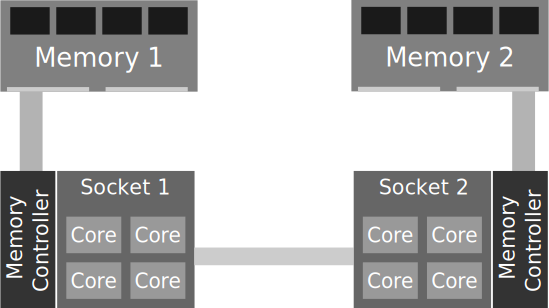
\includegraphics[width=3in]{alloc_numa_nb}
  \caption{NUMA Machine with 2 sockets of 4 cores}
  \label{fig:alloc_numa}
\end{figure}

In a general way, a program allocates memory from a virtual address space
split into pages. Each page used by the program is transparently
mapped to a physical memory location. Thus, some virtual pages can
also be moved from one physical location to another one, while the
virtual/physical mapping is transparently updated accordingly to the
operating system without affecting the execution of user level
programs. However, the physical location of virtual page may
impact the program performance on NUMA architectures, depending on the
connectivity between the physical memory bank where a page is
located and the socket core that is accessing this memory bank.

The NUMA memory allocation policy is defined by the operating system.
With Linux, at least the following three memory policies are generally available:
% CR: Add ``based operating systems'' after Linux ?
\begin{itemize}
\item {\em First Touch}: Memory is allocated on the bank next to
  the core which accessed the data first. This is the default policy.
\item {\em Bind}: Memory is allocated on a specific bank.
\item {\em Interleaved}: Memory allocations are interleaved among
  all the banks available.
\end{itemize}
On Linux, these policies can be set either through the
\textit{mbind} system call, or with the {\em numactl} command line tool.

Other operating system may come with their own specific sets of NUMA
memory allocation policies. Solaris, for instance, also provides the
\textit{next-touch}~\cite{next_touch}
% ST: TODO: Le papier de Brice & Nathalie n'est pas vraiment le mieux
% pour mentionner quelque chose de Solaris...
% CR: J'ai remplacé la citation par l'article cité par Brice & Nathalie dans \cite{GoFu09Next-touch}.
policy. When this policy is
selected, a memory page is moved to the bank close to
the core that subsequently accesses it.

%-------------------------------
\subsection{Interleaved Memory Allocation Policy}\label{subsec:numa_inter}
When the interleaved policy is selected, Linux uniformly distributes
newly allocated physical pages among all available NUMA banks,
following a round robin scheme. While having very little impact on the
applicative code, the interleave policy often shows some effectiveness
in mitigating NUMA overheads in the general case, because it
distributes the required memory bandwidth over the various memory banks.
Thus, it is usually
worthwhile to experiment with it, before investigating the NUMA issue
further.

The following tables show the performance results obtained after
enabling the interleaved memory allocation policy. We first test this
method using Intel TBB as the low-level runtime under the Taggre layer described in previous section
(Tables~\ref{tab:full:8:facto:no}~to~\ref{tab:full:8:solve:nested}).



While the results we obtain show an improved speed-up with TBB and interleaved policy,
it should be noted that sequential runs with interleaved policy are of
course worse, because of memory access penalties introduced by NUMA.
%% Parallel runs however show a better speed-up.
When comparing
interleaved page allocation with first-touch allocation, we get
an average improvement of 3.5\,\% on ILU(k) preconditioner
and 6.2\,\% on triangular solve with two 4-core sockets.

\begin{table}[!h]
  \renewcommand{\arraystretch}{1.3}
  \caption{Results on the ILU(k) factorization step on two 4-core sockets in natural ordering.}
  \label{tab:full:8:facto:no}
  \centering
  \begin{tabular}{|c|c||c|c|c|}
    \hline
    Matrix & ILU & TBB & TBB interleaved & Nas\\
    &     &  \multicolumn{3}{c|}{speed-up}\\
    \hline
    \hline
    & ILU(0) &            2.54  &  2.68  &  2.80\\
    CUBE\_100 & ILU(1) & 3.79  &  3.86  &  3.95\\
    & ILU(2) &            3.91  &  5.82  &  {\bf 6.19}\\
    \hline
    & ILU(0) &            3.78  &  5.10  &  5.34\\
    SPE10 &     ILU(1) &  5.72  &  5.84  &  6.64\\
    & ILU(2) &            6.21  &  6.34  &  {\bf 6.84}\\
    \hline
  \end{tabular}
\end{table}

\begin{table}[!h]
  \renewcommand{\arraystretch}{1.3}
  \caption{Results on the ILU(k) preconditioner step on two 4-core sockets in nested dissection ordering.}
  \label{tab:full:8:facto:nested}
  \centering
  \begin{tabular}{|c|c||c|c|c|c|}
    \hline
    Matrix & ILU & TBB & TBB interleaved & Nas\\
    &     &  \multicolumn{3}{c|}{speed-up}\\
    \hline
    \hline
    & ILU(0) &            3.31  &  3.65  &  3.95\\
    CUBE\_100 & ILU(1) &  4.77  &  4.90  &  5.14\\
    & ILU(2) &            5.46  &  5.54  &  {\bf 5.72}\\
    \hline
    & ILU(0) &            3.09  &  3.70  &  4.00\\
    SPE10     & ILU(1) &  5.00  &  5.01  &  5.57\\
    & ILU(2) &            5.57  &  5.62  &  {\bf 6.06}\\
    \hline
  \end{tabular}
\end{table}



\begin{table}[!h]
  \renewcommand{\arraystretch}{1.3}
  \caption{Results on the Triangular Solve step on two 4-core sockets in natural ordering.}
  \label{tab:full:8:solve:no}
  \centering
  \begin{tabular}{|c|c||c|c|c|c|}
    \hline
    Matrix & ILU & TBB & TBB interleaved & Nas\\
    &     &  \multicolumn{3}{c|}{speed-up}\\
    \hline
    \hline
    & ILU(0) &            2.44  &  3.51  &  2.66\\
    CUBE\_100 & ILU(1) &  2.82  &  3.68  &  2.95\\
    & ILU(2) &            2.98  &  {\bf 3.76}  &  3.18\\
    \hline
    & ILU(0) &            2.52  &  3.58  &  3.24\\
    SPE10     & ILU(1) &  3.77  &  4.04  &  4.43\\
    & ILU(2) &            4.14  &  4.41  &  {\bf 4.96}\\
    \hline
  \end{tabular}
\end{table}

\begin{table}[!h]
  \renewcommand{\arraystretch}{1.3}
  \caption{Results on the Triangular Solve step on two 4-core
    sockets with TBB and interleaved allocation with nested dissection.}
  \label{tab:full:8:solve:nested}
  \centering
  \begin{tabular}{|c|c||c|c|c|c|}
    \hline
    Matrix & ILU & TBB & TBB interleaved & Nas\\
    &     &  \multicolumn{3}{c|}{speed-up}\\
    \hline
    \hline
    & ILU(0) &            1.67  &  2.11  &  1.92\\
    CUBE\_100 & ILU(1) &  1.92  &  2.25  &  2.07\\
    & ILU(2) &            2.08  &  {\bf 2.42}  &  2.24\\
    \hline
    & ILU(0) &            1.82  &  2.26  &  2.19\\
    SPE10     & ILU(1) &  2.71  &  2.82  &  3.08\\
    & ILU(2) &            2.90  &  3.01  &  {\bf 3.32}\\
    \hline
  \end{tabular}
\end{table}

These improvements could be further enhanced by taking into account the locality of data 
used by tasks within the task scheduler. This is the purpose of the
following section.


%=========================================================
\section{NUMA Aware Scheduling}\label{sec:numa_sched}
%=========================================================
In order to easily experiment with NUMA-aware task scheduling, we
implemented our own basic NUMA task scheduler. We call this scheduler
``Nas'' (NUMA Aware Scheduler) in the remainder of this paper. 

Nas design is similar to TBB, in that, tasks are objects containing an execute
method and some extra information such as dependencies.
We add NUMA node affinity into tasks objects to allow Nas scheduling
tasks with the best affinity. This NUMA affinity can be strict or not.
In strict mode, the tasks can only be executed on one NUMA node. In flexible
mode, tasks are executed in priority on the specified NUMA, but can also be
executed somewhere else if needed.

In Nas, threads of the same NUMA node share the same container of tasks, unlike
other runtimes that use one deque per thread. When a
task becomes available, it is put into the container corresponding to
its NUMA affinity if set,
otherwise a round robin algorithm is used by default. Because of thread concurrency
over the container, we didn't choose a simple deque but rather an optimized
structure which allows multiple operations at the same time.

Nas also provides control over data allocation and distribution
among NUMA banks, as well as memory block moves among NUMA banks.

Nas and Taggre are designed to cooperate together, with Taggre being
responsible for the DAG preprocessing, and Nas acting as the
runtime back-end. Both tools also cooperate together in controlling the placement of
tasks on the NUMA platform: The aggregation operator is called using
the Front algorithm with the number of NUMA nodes as parameter.

%-------------------------------
\subsection{NUMA helpers}
\label{NUMA_helper}
Nas has some NUMA helpers. The first helper is a function to allocate data
and distribute it over all NUMA banks. This is equivalent to starting a static
parallel for with OpenMP and First Touch policy activated, but in our case we have simplified this through a single function call. 
This helper is mainly useful for vector allocation.

The second helper is a function to move data between NUMA banks. The user registers the piece
of data and where he wants to move it. This helper is basically a wrapper for
the {\em move\_pages} system call. It automatically splits memory address and size into
a set of memory addresses aligned to page boundaries. This helper can be combined with Taggre
to distribute data by taking into account data access over computation time.
Thus, using Nas in conjunction with Taggre is a very convenient way to manage NUMA seamlessly in a task driven parallelization. 
Indeed, we provide a single function that uses the Taggre DAG to perform
an allocate or move memory pages of the data in order to balance the
work between sockets in accordance with the DAG. 
The task affinity with the sockets where its data are allocated is then
used by the scheduler to minimize the NUMA penalties. More details are
given in the next section.

%-------------------------------
\subsection{Nas with Taggre}
In order to optimize memory distribution, one can use the DAG of Taggre, and
Nas as runtime.
In most cases, tasks have data from other tasks to read in input and produce data
for other tasks in output. By distributing tasks over NUMA nodes, we can indirectly distribute
the data production. In most cases, the NUMA penalty of a write access is worst than
the NUMA penalty of a read access. The tasks distribution is done with the Front algorithm
and the number of NUMA nodes as parameter (Fig. \ref{fig:distrib_numa}).

Then we need to match the NUMA locality of data with the NUMA affinity of tasks which use it
by moving physical pages on the right NUMA bank.
To do this, we simulate an execution of the DAG with a user defined function. This
function is called for each task and must register data write in the
task to express that it should be brought them closer. 

In the case of GMRES, we distribute the row of the matrix following the DAG. All
vectors used during triangular solve are allocated using the first NUMA helper.


\begin{figure}[!t]
  \centering
  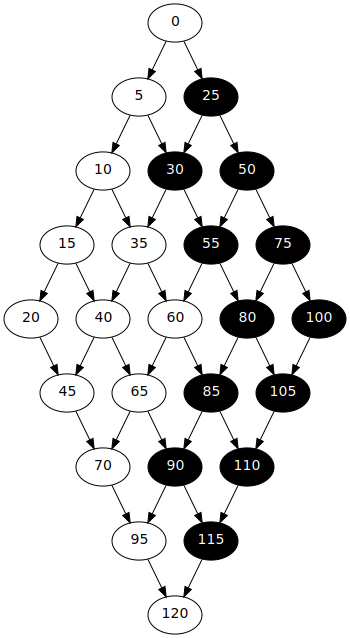
\includegraphics[width=2.5in]{numa_distrib}
  \caption{Distribution of tasks between 2 NUMA nodes, in white tasks of node 1, in black tasks of node 2}
  \label{fig:distrib_numa}
\end{figure}

%-------------------------------
\subsection{Result}
On a single 4-core socket, the Nas scheduler delivers results very similar to those
of TBB because no NUMA is involved. On our NUMA platform with two 4-core sockets,
the Nas scheduler delivers better results than TBB. On the
factorization step, we achieve an improvement
from 1 to 40\,\% (Tables~\ref{tab:full:8:facto:no},~\ref{tab:full:8:facto:nested}).

On the triangular solve step, the
improvement obtained with the Nas scheduler is 12.36\,\% on average
(Tables~\ref{tab:full:8:solve:no},~\ref{tab:full:8:solve:nested}). 
%% On Cube\_100 case, interleaved method is more effective than Nas method because of memory access
%% to the vector. For now, we allocate the vector with the first NUMA helper of Nas,
%% but during triangular solve, the first part of the vector is only write by first NUMA node, then
%% gradually the second NUMA node interleave some write in the middle part of the vector and finally only the second NUMA node
%% write the end of the vector. We are working on a generic way to optimize memory distribution.

On Cube\_100 case, one can notice that the interleaved memory allocation method
gives better results than using our NUMA aware allocator. This is due to the fact
that in the triangular solve, a task accesses the matrix data and some part of
the vector. The problem is that the matrix is allocated using the second NUMA helper
allocator (described in Subsection \ref{NUMA_helper}) whereas the vector is
allocated using the first NUMA helper allocator (optimized for the matrix-vector
product). Hence, the memory accesses to the vector are not optimized in the
triangular solve and the interleaved memory allocation method gives better results
in average. One can see that in the case SPE10 where each entry of the matrix
is a dense block (3,3), the memory accesses to the vector are more neglectable
and in this case the NUMA allocator is better.


%% \begin{table}[!h]
%%   \renewcommand{\arraystretch}{1.3}
%%   \caption{Results on the ILU(k) factorization step on two 4-core
%%     sockets with Nas with natural ordering}
%%   \label{tab:nas:8:facto:no}
%%   \centering
%%   \begin{tabular}{|c|c||c|c|}
%%     \hline
%%     Matrix & ILU & CD(4) & Improvement\\
%%     &     &  (speed-up) & compare to TBB\\
%%     \hline
%%     \hline
%%     & ILU(0) & 2.80 & 7.86\,\%\\
%%     CUBE\_100 & ILU(1) & 3.95 & 2.34\,\%\\
%%     & ILU(2) & 6.19 & 20.51\,\%\\
%%     \hline
%%     & ILU(0) & 5.34 & 39.77\,\%\\
%%     SPE10     & ILU(1) & 6.64 & 14.27\,\%\\
%%     & ILU(2) & 6.84 & 7.30\,\%\\
%%     \hline
%%   \end{tabular}
%% \end{table}
%% \begin{table}[!h]
%%   \renewcommand{\arraystretch}{1.3}
%%   \caption{Results on the ILU(k) factorization step on two 4-core
%%     sockets with Nas with nested dissection}
%%   \label{tab:nas:8:facto:nested}
%%   \centering
%%   \begin{tabular}{|c|c||c|c|}
%%     \hline
%%     Matrix & ILU & D(400) & Improvement\\
%%     &     &  (speed-up) & compare to TBB\\
%%     \hline
%%     \hline
%%     & ILU(0) & 3.95 & 17.56\,\%\\
%%     CUBE\_100 & ILU(1) & 5.14 & 2.24\,\%\\
%%     & ILU(2) & 5.72 & 1.00\,\%\\
%%     \hline
%%     & ILU(0) & 4.00 & 31.70\,\%\\
%%     SPE10     & ILU(1) & 5.57 & 8.72\,\%\\
%%     & ILU(2) & 6.06 & 6.49\,\%\\
%%     \hline
%%   \end{tabular}
%% \end{table}


%% \begin{table}[!h]
%%   \renewcommand{\arraystretch}{1.3}
%%   \caption{Results on the Triangular Solve step on two 4-core
%%     sockets with Nas with natural ordering}
%%   \label{tab:nas:8:solve:no}
%%   \centering
%%   \begin{tabular}{|c|c||c|c|}
%%     \hline
%%     Matrix & ILU & CD(4) & Improvement\\
%%     &     &  (speed-up) & compare to TBB\\
%%     \hline
%%     \hline
%%     & ILU(0) & 2.66 & 7.55\,\%\\
%%     CUBE\_100 & ILU(1) & 2.95 & 3.67\,\%\\
%%     & ILU(2) & 3.18 & 4.85\,\%\\
%%     \hline
%%     & ILU(0) & 3.24 & 26.68\,\%\\
%%     SPE10     & ILU(1) & 4.43 & 16.62\,\%\\
%%     & ILU(2) & 4.96 & 19.07\,\%\\
%%     \hline
%%   \end{tabular}
%% \end{table}

%% \begin{table}[!h]
%%   \renewcommand{\arraystretch}{1.3}
%%   \caption{Results on the Triangular Solve step on two 4-core
%%     sockets with Nas with nested dissection}
%%   \label{tab:nas:8:solve:nested}
%%   \centering
%%   \begin{tabular}{|c|c||c|c|}
%%     \hline
%%     Matrix & ILU & D(400) & Improvement\\
%%     &     &  (speed-up) & compare to TBB\\
%%     \hline
%%     \hline
%%     & ILU(0) & 1.92 & 14.49\,\%\\
%%     CUBE\_100 & ILU(1) & 2.07 & 7.02\,\%\\
%%     & ILU(2) & 2.24 & 6.73\,\%\\
%%     \hline
%%     & ILU(0) & 2.19 & 18.71\,\%\\
%%     SPE10     & ILU(1) & 3.08 & 12.49\,\%\\
%%     & ILU(2) & 3.32 & 13.42\,\%\\
%%     \hline
%%   \end{tabular}
%% \end{table}



%=========================================================
\section{Conclusions and Future Work}\label{sec:conclusion}
%=========================================================
\input{chapter_conclusion}

\bibliography{ipdps}


% that's all folks
\end{document}

























































% for over three affiliations, or if they all won't fit within the width
% of the page, use this alternative format:
% 
%\author{\IEEEauthorblockN{Michael Shell\IEEEauthorrefmark{1},
%Homer Simpson\IEEEauthorrefmark{2},
%James Kirk\IEEEauthorrefmark{3}, 
%Montgomery Scott\IEEEauthorrefmark{3} and
%Eldon Tyrell\IEEEauthorrefmark{4}}
%\IEEEauthorblockA{\IEEEauthorrefmark{1}School of Electrical and Computer Engineering\\
%Georgia Institute of Technology,
%Atlanta, Georgia 30332--0250\\ Email: see http://www.michaelshell.org/contact.html}
%\IEEEauthorblockA{\IEEEauthorrefmark{2}Twentieth Century Fox, Springfield, USA\\
%Email: homer@thesimpsons.com}
%\IEEEauthorblockA{\IEEEauthorrefmark{3}Starfleet Academy, San Francisco, California 96678-2391\\
%Telephone: (800) 555--1212, Fax: (888) 555--1212}
%\IEEEauthorblockA{\IEEEauthorrefmark{4}Tyrell Inc., 123 Replicant Street, Los Angeles, California 90210--4321}}






% An example of a floating table. Note that, for IEEE style tables, the 
% \caption command should come BEFORE the table. Table text will default to
% \footnotesize as IEEE normally uses this smaller font for tables.
% The \label must come after \caption as always.
%
%\begin{table}[!t]
%% increase table row spacing, adjust to taste
%\renewcommand{\arraystretch}{1.3}
% if using array.sty, it might be a good idea to tweak the value of
% \extrarowheight as needed to properly center the text within the cells
%\caption{An Example of a Table}
%\label{table_example}
%\centering
%% Some packages, such as MDW tools, offer better commands for making tables
%% than the plain LaTeX2e tabular which is used here.
%\begin{tabular}{|c||c|}
%\hline
%One & Two\\
%\hline
%Three & Four\\
%\hline
%\end{tabular}
%\end{table}





% use section* for acknowledgement
%\section*{Acknowledgment}
%The authors would like to thank...
%more thanks here







% trigger a \newpage just before the given reference
% number - used to balance the columns on the last page
% adjust value as needed - may need to be readjusted if
% the document is modified later
%\IEEEtriggeratref{8}
% The "triggered" command can be changed if desired:
%\IEEEtriggercmd{\enlargethispage{-5in}}

%% \begin{figure}[!t]
%%   \centering
%%   \subfloat[Case I]{\includegraphics[width=0.20\textwidth]{pics/diamond.png}\hfil}
%%   \subfloat[Case II]{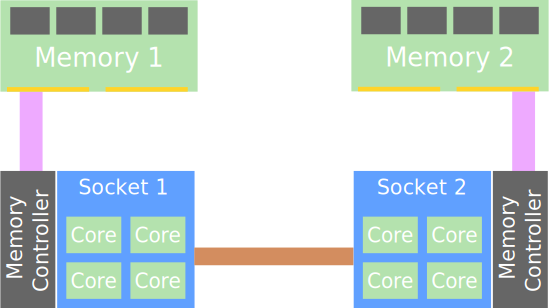
\includegraphics[width=0.20\textwidth]{pics/alloc_numa.pdf}\hfil}
%% \caption{Simulation results}
%% \label{fig_sim}
%% \end{figure}
